%  article.tex (Version 3.3, released 19 January 2008)
%  Article to demonstrate format for SPIE Proceedings
%  Special instructions are included in this file after the
%  symbol %>>>>
%  Numerous commands are commented out, but included to show how
%  to effect various options, e.g., to print page numbers, etc.
%  This LaTeX source file is composed for LaTeX2e.

%  The following commands have been added in the SPIE class 
%  file (spie.cls) and will not be understood in other classes:
%  \supit{}, \authorinfo{}, \skiplinehalf, \keywords{}
%  The bibliography style file is called spiebib.bst, 
%  which replaces the standard style unstr.bst.  

\documentclass[]{spie}  %>>> use for US letter paper
%%\documentclass[a4paper]{spie}  %>>> use this instead for A4 paper
%%\documentclass[nocompress]{spie}  %>>> to avoid compression of citations
%% \addtolength{\voffset}{9mm}   %>>> moves text field down
%% \renewcommand{\baselinestretch}{1.65}   %>>> 1.65 for double spacing, 1.25 for 1.5 spacing 
%  The following command loads a graphics package to include images 
%  in the document. It may be necessary to specify a DVI driver option,
%  e.g., [dvips], but that may be inappropriate for some LaTeX 
%  installations. 
\usepackage[]{graphicx}
\usepackage{url}

\title{SLI in AR applications} 

%>>>> The author is responsible for formatting the 
%  author list and their institutions.  Use  \skiplinehalf 
%  to separate author list from addresses and between each address.
%  The correspondence between each author and his/her address
%  can be indicated with a superscript in italics, 
%  which is easily obtained with \supit{}.

\author{Daniel L. Lau\supit{a} and Ying Yu\supit{a} and Matthew P. Ruffner\supit{a}
\skiplinehalf
\supit{a}University of Kentucky, Address, Lexington, US; \\
%\supit{b}University of Kentucky, Address, Lexington, US
}

%>>>> Further information about the authors, other than their 
%  institution and addresses, should be included as a footnote, 
%  which is facilitated by the \authorinfo{} command.

\authorinfo{Further author information: (Send correspondence to A.A.A.)\\A.A.A.: E-mail: aaa@tbk2.edu, Telephone: 1 505 123 1234\\  B.B.A.: E-mail: bba@cmp.com, Telephone: +33 (0)1 98 76 54 32}
%%>>>> when using amstex, you need to use @@ instead of @
 

%%%%%%%%%%%%%%%%%%%%%%%%%%%%%%%%%%%%%%%%%%%%%%%%%%%%%%%%%%%%% 
%>>>> uncomment following for page numbers
% \pagestyle{plain}    
%>>>> uncomment following to start page numbering at 301 
%\setcounter{page}{301} 
 
  \begin{document} 
  \maketitle 

%%%%%%%%%%%%%%%%%%%%%%%%%%%%%%%%%%%%%%%%%%%%%%%%%%%%%%%%%%%%% 
\begin{abstract}
This document shows the desired format and appearance of a manuscript prepared for the Proceedings of the SPIE.  It contains general formatting instructions and hints about how to use LaTeX.  The LaTeX source file that produced this document, {\tt article.tex} (Version 3.3), provides a template, used in conjunction with {\tt spie.cls} (Version 3.3).  
\end{abstract}

%>>>> Include a list of keywords after the abstract 

\keywords{Manuscript format, template, SPIE Proceedings, LaTeX}

%%%%%%%%%%%%%%%%%%%%%%%%%%%%%%%%%%%%%%%%%%%%%%%%%%%%%%%%%%%%%
\section{INTRODUCTION}
\label{sec:intro}  % \label{} allows reference to this section
Structured light illumination is a 3D scanning technique based on projecting a series of striped line patterns and then reconstructing a target surface based on the warping of the stripes as measured by a digital camera~\cite{lieb05}.  Compared to alternative schemes like passive stereovision~\cite{curl96} or time-of-flight~\cite{gokt04}, structured light is far superior in terms of accuracy~\cite{lijl03}, but as a triangulation scheme, SLI cannot easily scan at long ranges~\cite{anyt16}.  Furthermore, as a scanning process, SLI is not typically associated with real-time applications with moving targets~\cite{deet17}.

Scanning time is a major issue in structured light research as numerous papers have been published that focus either on using high speed projector/camera pairs~\cite{gong10} or using unique pattern codecs~\cite{zhan04, suwh06,liuk10} that minimize the number of projected patterns. In fact, single pattern SLI techniques do exist~\cite{take83, wust91, koni06} that are quite popular in human computer interfacing applications~\cite{guan05} but which perform poorly in bright ambient light conditions~\cite{yuan12}. 

With regards to performing structured light scanning with commodity components, a major issue is the inability to properly synchronize a camera and projector such that one can associate a specific pattern to a specific captured image without including some type of key-frame scheme and analyzing the pixels of the captured image. As clearly documented by graphics card manufacturers, GPUs are not real-time systems, and there is no way for the CPU to know when a requested pattern shows up on the HDMI port~\cite{nvid18}. And while it is possible to guarantee that no particular pattern is dropped, it is not possible to guarantee that a particular pattern is not repeated multiple times in a row.

As a means of addressing one's ability to properly synchronize the camera and projector, there are commercially available projectors that include electronics to embed patterns into the projector which include appropriate GPIO to interface with a camera's trigger~\cite{glop18, ajil18, lcft18}; however, these projectors are inordinately expensive on a per lumens basis.  As of the time of this writing, the TI Lightcrafter 4500 retails for \$1,250 with only 150~lumens brightness~\cite{tilc17} while an LED-based Optoma ML750ST has approximately 500 lumens brightness~\cite{lume70} with the same spatial light modulator for \$550~\cite{ml75st}. Admittedly, the TI Lightcrafter 4500 can project patterns at up to 4,225~Hz, but the 120~Hz of 3D ready projectors is more than adequate for most machine vision cameras limited in frame rate by either the bus to the CPU (USB 3.0, for instance) or by the exposure time required by the sensor.

As a means of ensuring perfect projector/camera synchronization using commodity components, we propose a novel approach to machine vision camera architectures by incorporating HDMI pass-through where the camera reads the incoming HDMI video to extract hand-shaking messages embedded into the top-left pixel. Such handshaking could be used to then trigger the camera to capture the projected frames, ignoring duplicate or don't care frames.  Without an incoming HDMI signal, the machine vision camera can alternately produce its own video signal, converting any HDMI projector into an instant structured light scanner which it instantly syncs.  

Aside from simple synchronization to a projector, the incorporation of HDMI into a machine vision sensor produces many application possibilities. For instance, cameras could take advantage of EDID~\cite{edid00} to tell a host CPU what kind of camera it is and what its capabilities are including its resolution, color space, and frame rates.  Multiple cameras can also by daisy chained together and instantly synchronized together using commodity cables purchased at any big box store with cable lengths of 15, 25, or even 50 feet~\cite{hdmi50} or longer with appropriate repeaters~\cite{repe00}. And now with the inclusion of ethernet over HDMI~\cite{hdmi14}, one could easily see GigE cameras converted to HDMI in the near future.

Now an application for our HDMI pass-through cameras that we are particularly interested is projector-based augmented reality such as the AR Sandbox~\cite{wood16} and the AR Pool Table~\cite{uchi08}. In the case of the AR Sandbox, a digital projector paired with a PrimeSense RGB+D camera with the RGB+D camera used to monitor the shape of sand in a sandbox placed under the projector as depicted in Fig.~\ref{??}.  The shape of the sand is then used to generate a psuedo-color relief map which is then projected back onto the sand in perfect register.  The result system can then be used to visualize water flow through simulated rivers and streams~\cite{afro18}.  

In the AR Pool Table, a digital projector is used to direct the player on where and how to strike the que ball in order to sink the other balls in the various pockets.  A machine vision camera monitors the balls' positions on the table as well as the pose of the stick and project augmenting lines onto the table in order to show the player how well their stick alignment matches the alignment posed by the CPU.  Working in reverse, the AR Pool Table is now being used to train the PC the play pool using a robotic stick~\cite{gree08}.

In either of the above or other projector-based AR systems~\cite{miya11, kemm16, dosh17}, a common trait of all systems is their inclusion of low-accuracy 3D vision with a commodity projector.  Our proposed machine vision camera with HDMI pass through could be instantly inserted between the projector and computer to give that system the option of highly accurate (millimeter) 3D scanning when the RGB+D sensors give only centimeter accuracy. Such high resolution would not only enhance scene understanding in the computer (having highly accurate scans) but also enhance registration between the target surface with the projector as the camera can derive sub-pixel alignment with the projector.

%\section{HDMI and EDID}
%As mentioned earlier, the graphics cards are not real-time, driving the projector directly from the graphics card is not feasible. So we built a dedicated FPGA-based HDMI controller to synchronize the projector with the camera. The HDMI bus does not transfer video data all the time, in fact, there are some windows. The video data are transferred only during these windows. Take a video of $800 \times 600$ resolution for example, each frame is devided into 600 rows,  each row has 800 pixels. All these 800 pixels are considered as one group, each group is operated as an entirety, in other words, any 800 pixels in a same row are transferred at a time without any interruptions,here we call this period horizontal active pixels time. But in between any two successive rows, there are intervals during which no video data are being sent. This blank period includes three distinct phases, they are measured in the unit of pixel clock cycle and are usually referred to as horizontal front porch (HFP), horizontal sync pulse (HSP) and horizontal back porch (HBP). Similarly the HDMI organizes a frame of image in a certain number of rows which in this case is 600. It treats 600 rows as a whole and between every two successive frames, there is an interval consists of vertical front porch (VFP), vertical sync pulse (VSP) and vertical back porch (VBP). Instead of pixel clock, they are measured in the unit of row cycle.  Figure \ref{Fig:1} illustrates the principle of the above HDMI timing.
%Since the periods of VSync being high is the actual window when a whole frame is transferred, the VSync is one of the important signals that are needed in synchronization with camera. Although VSync is not a separate wire in a standard HDMI bus, by deserializing and decoding the data stream in blue channel of the HDMI bus, three control signals,  $HSync$, $VSync$ and $DE$ can be extracted. The $DE$ signal is a series of windows where each windows represents the transferal of a row of active pixels, it can be defined as, 
% \begin{equation} \label{}
%  	DE = H.Active Pixels \& V. Active Pixels,
%  \end{equation}
%The structured light patterns we apply in our system are the phase-shifting sinusoidal patterns, it is not enough to merely know the start and end points of a frame, but it is also important to know which pattern is to be projected next. We developed a scheme to encode some index information in the pattern itself while not  affecting the 3D measurement. A unique index value of the pattern is set as the color value of the top left pixel which is also the very first pixel of a frame. Therefore the HDMI controller identifies which pattern it is by reading the first pixel.To locate the first pixel, the $DE$ signal becomes quite crutial. The first rising edge of the $DE$ after the rising edge of $V.Active Pixels$ indicates the beginning of the first row, and the first pixel clock after the beginning of the first row points to the first pixel in a frame.

%\begin{figure}
%   \begin{center}
%   \begin{tabular}{c}
%   %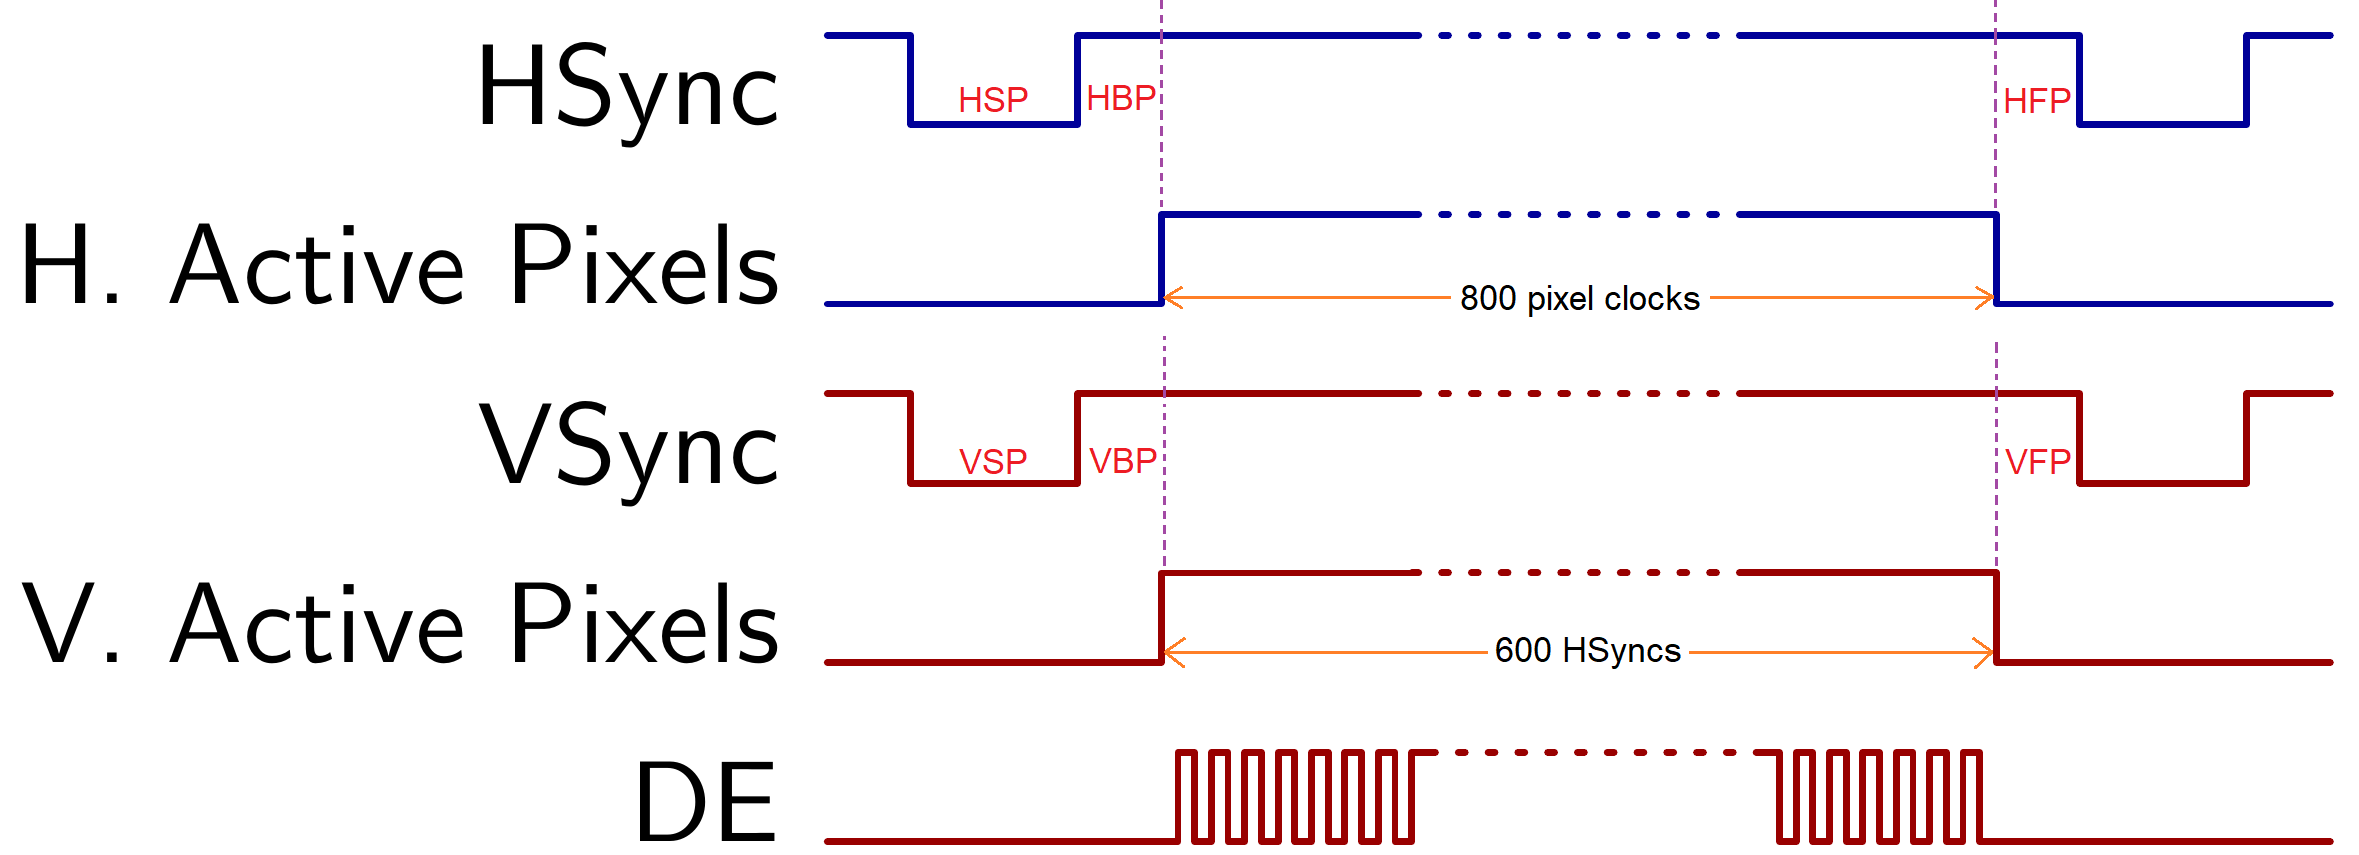
\includegraphics[height=7cm]{wf3.png}
%   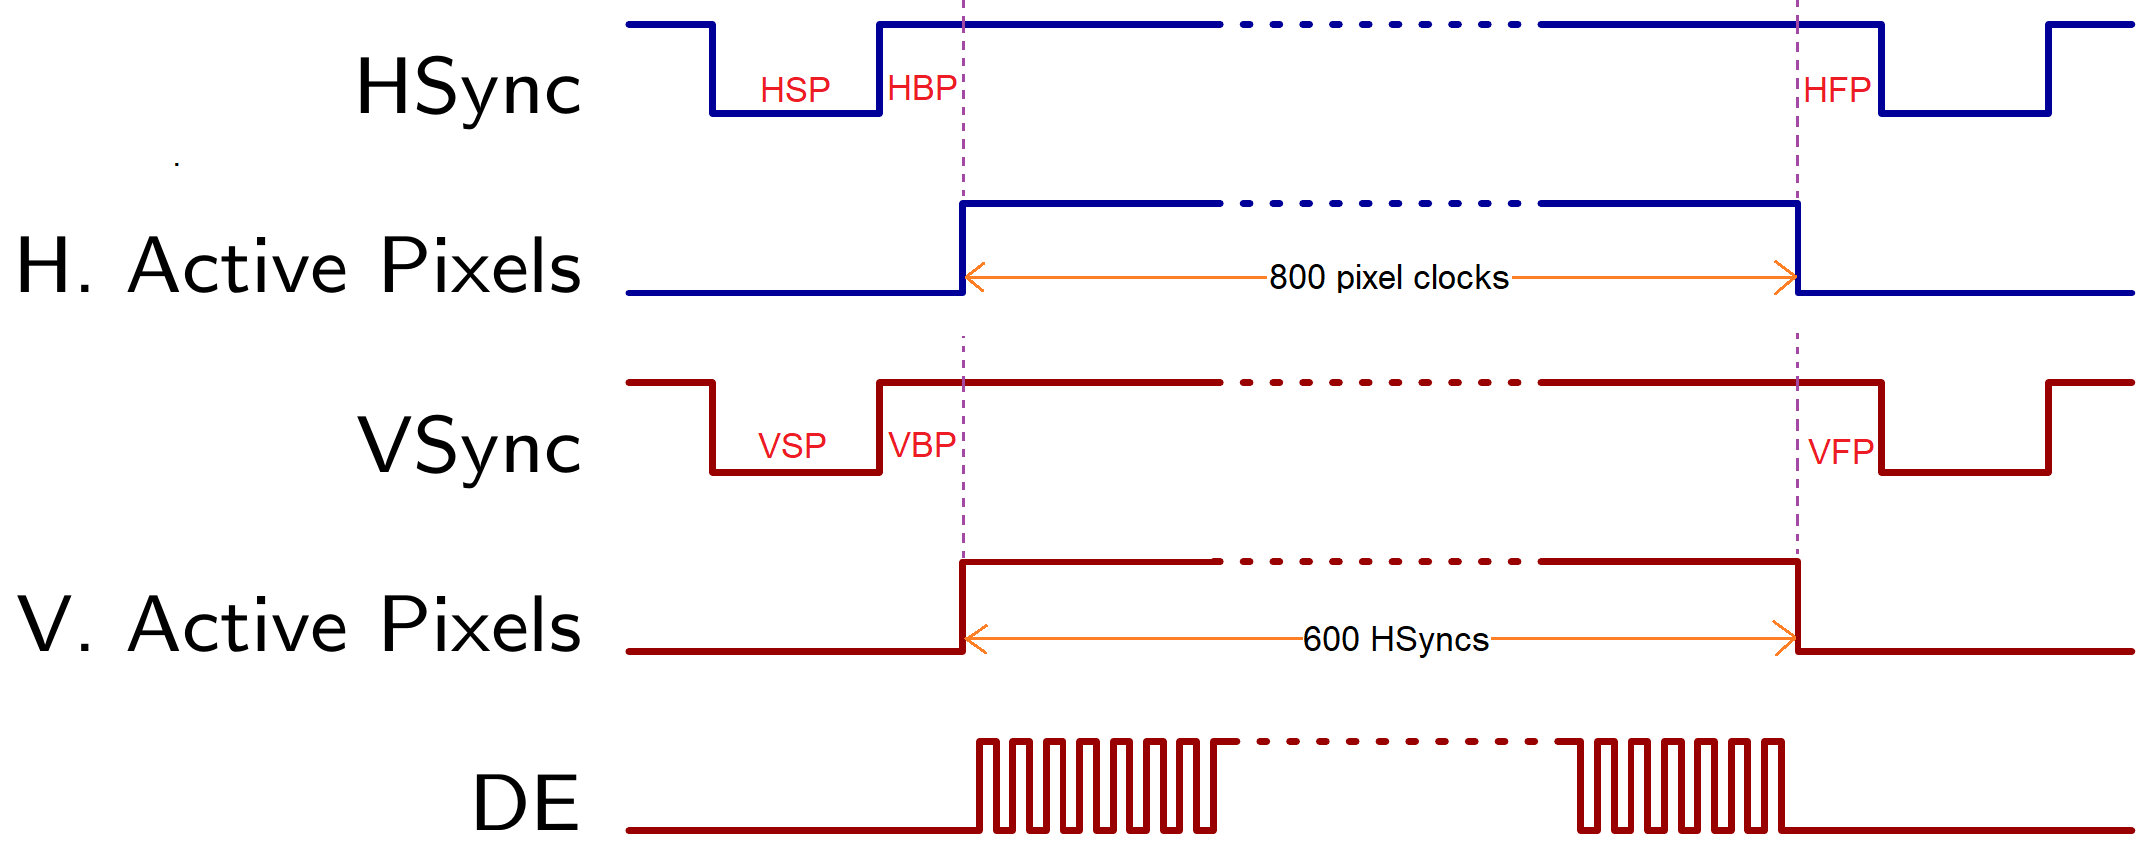
\includegraphics[width=0.8\linewidth]{wf1.png} 
%   \end{tabular}
%   \end{center}
%   \caption{HDMI timing}%[HDMI timing] >>>> use \label inside caption to get Fig. number with \ref{}
%   \label{Fig:1}% Figure captions are used to describe the figure and help the reader understand it's significance.  The caption should be centered underneath the figure and set in 9-point font.  It is preferable for figures and tables to be placed at the top or bottom of the page. LaTeX tends to adhere to this standard.}
%   \end{figure} 

%Unlike the VGA port which automatically starts data transferring upon plug-in, the HDMI protocol adds an initial handshake process via $I^2C$ bus in its DDC channel before the video data transferal. In the process, the HDMI source sends an $I^2C$ based command on detecting a hot plug signal from an HDMI sink device. After receiving a command at slave address $0xA0$, the sink which is the HDMI controller in our case, starts to send the 128-byte or 256-byte EDID data to source. The EDID contains various information about the HDMI sink, including the manufacturer ID, serial number, year of manufacture, EDID version and revision, etc. More importantly, the supported resolutions and refresh rates of the sinks, even the detailed timing such as pixel clock frequency, HFP, VFP, HBP, VBP, HSP, VSP are part of the EDID. Being able to define and encode these parameters in EDID allows us to run the system at any customized resolutions as well as any refresh rates. We created our own EDID by incorporating an $I^2C$ slave controller in the FPGA.

\section{Hardware structure}
The entire system is based on a Zynq 7000 SoC. The Zynq 7000 consists of two parts, processing system (PS) and programmable logic (PL). PS is dual-core ARM Cortex-A9 processor, and PL is equivalent to a Xilinx 7 series FPGA. After powering on, an 80Mhz clock signal from the PL is not immediately fed to the LUPA300 until the PS boots up the operating system and configures the PL. However, the LUPA300 requires that the clock is supplied earlier than the power and the reset, so a delay logic is necessary to make sure that the power is supplied after the clock.
Meanwhile, an EDID simulator is set to standby in the DDC channel of the HDMI once the PL is configured. Upon receiving an EDID request from the PC, it responses with a 128-byte or 256-byte EDID data package. Once this data is recognized by the PC, PC starts to streams video to the PL through the HDMI cable. In this case, the PL just passes whatever it receives to the projector. On the other hand, if the the PL doesn't detect a clock from the PC in 3 seconds, which indicates that there's no valid HDMI connection, a multiplexer will route the structured light patterns generated by the SLI pattern generator to the projector. The SLI pattern generator has its clock from an external oscillator (Si514). On the LUPA300 side, there is a control logic which includes a SPI controller and a synchronization module. The SPI controller configures the LUPA300 on startup by loading a bunch of internal registers with user defined values through a SPI bus. The synchronization module synchronizes the LUPA300 with a Vertical Sync signal either from the PC or the SLI pattern generator. To start a scan, the PC issues a command to the PS via Ethernet, the command as well as two parameters, exposure time and trigger delay are sent to the PL via Xillybus which is a dedicated IP core that provides some APIs for FPGA and Linux operating system to communicate. Then the PL begins to trigger the LUPA300 according to these parameters along with the synchronization module. After that the output data bus of the LUPA300 sequentially transmits pixel data to the FIFO, the Xillybus, the PS, and eventually the host PC. Fig.~\ref{Fig:3} illustrates the system diagram discussed above.

\begin{figure}{!t}
   \begin{center}
   \begin{tabular}{c}
   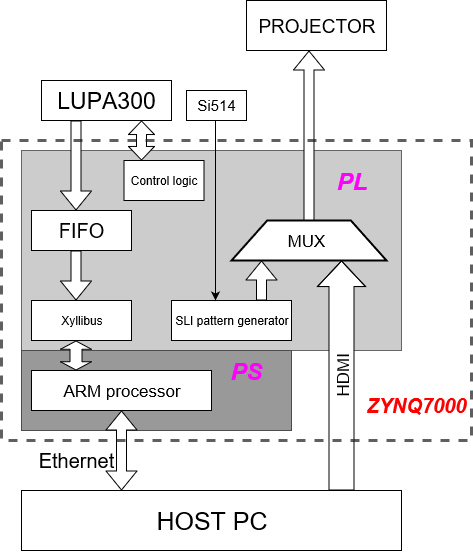
\includegraphics[height=7cm]{ardg.png} 
   \end{tabular}
   \end{center}
   \caption{System diagram}
   \label{Fig:3}
   \end{figure} 

 
%This document shows the desired format and appearance of a manuscript prepared for the Proceedings of the SPIE.\footnote{The basic format was developed in 1995 by Rick Herman (SPIE) and Ken Hanson (Los Alamos National Lab.).} It is prepared using LaTeX2e\cite{Lamport94} with the class file {\tt spie.cls}.  The LaTeX source file used to create this document is {\tt article.tex}, which contains important formatting information embedded in it.  These files are available on the Internet at {\tt http://home.lanl.gov/kmh/spie/}.  The font used throughout is the LaTeX default font, Computer Modern Roman, which is equivalent to the Times Roman font available on many systems.  If this font is not available, use a similar serif font.  Normal text has a font size of 10 points\footnote{Font sizes are specified in points, abbreviated pt., which is a unit of length.  One inch = 72.27 pt.; one cm = 28.4 pt.} for which the actual height of a capital E is about 2.4 mm (7 pt.) and the line-to-line spacing is about 4.2 mm (12 pt.).  The font attributes for other parts of the manuscript, summarized in Table~\ref{tab:fonts}, are described in the following sections.  Normal text should be justified to both the left and right margins.  Appendix~\ref{sec:latex} has information about PostScript fonts.
%
%To be properly reproduced in the Proceedings, all text and figures must fit inside a rectangle 6.75-in.\ wide by 8.75-in.\ high or 17.15 cm by 22.23 cm.  The text width and height are set in {\tt spie.cls} to match this requirement.
%% This table is carefully placed in the source file to make 
%% it appear at bottom of page, but above the footnotes.  
%% Use of [h] in following command forces table to appear "here".
%\begin{table}[h]
%\caption{Fonts sizes to be used for various parts of the manuscript.  All fonts are Computer Modern Roman or an equivalent.  Table captions should be centered above the table.  When the caption is too long to fit on one line, it should be justified to the right and left margins of the body of the text.} 
%\label{tab:fonts}
%\begin{center}       
%\begin{tabular}{|l|l|} %% this creates two columns
%% |l|l| to left justify each column entry
%% |c|c| to center each column entry
%% use of \rule[]{}{} below opens up each row
%\hline
%\rule[-1ex]{0pt}{3.5ex}  Article title & 16 pt., bold, centered  \\
%\hline
%\rule[-1ex]{0pt}{3.5ex}  Author names and affiliations & 12 pt., normal, centered   \\
%\hline
%\rule[-1ex]{0pt}{3.5ex}  Section heading & 11 pt., bold, centered (all caps)  \\
%\hline
%\rule[-1ex]{0pt}{3.5ex}  Subsection heading & 11 pt., bold, left justified  \\
%\hline
%\rule[-1ex]{0pt}{3.5ex}  Sub-subsection heading & 10 pt., bold, left justified  \\
%\hline
%\rule[-1ex]{0pt}{3.5ex}  Normal text & 10 pt., normal  \\
%\hline
%\rule[-1ex]{0pt}{3.5ex}  Figure and table captions & \, 9 pt., normal \\
%\hline
%\rule[-1ex]{0pt}{3.5ex}  Footnote & \, 9 pt., normal \\
%\hline 
%\end{tabular}
%\end{center}
%\end{table} 
%The text should begin 1.00 in.\ or 2.54 cm from the top of the page.  The right and left margins should be 0.875~in.\ or 2.22 cm for US letter-size paper (8.5 in.\ by 11 in.) or 1.925 cm for A4 paper (210 mm by 297 mm) to horizontally center the text on the page.  See Appendix~\ref{sec:latex} for guidance regarding paper-size specification. 
%
%Authors are encouraged to follow the principles of sound technical writing, as described in Refs.~\citenum{Alred03} and \citenum{Perelman97}, for example.  Many aspects of technical writing are addressed in the {\em AIP Style Manual}, published by the American Institute of Physics.  It is available on line at {\tt http://www.aip.org/pubservs/style/4thed/toc.html} or {\tt http://public.lanl.gov/kmh/AIP\verb+_+Style\verb+_+4thed.pdf}. A spelling checker is helpful for finding misspelled words. 
%
%An author may use this LaTeX source file as a template by substituting his/her own text in each field.  This document is not meant to be a complete guide on how to use LaTeX.  For that, refer to books on LaTeX usage, such as the definitive work by Lamport\cite{Lamport94} or the very useful compendium by Mittelbach et al.\cite{Mittelbach04}

%%%%%%%%%%%%%%%%%%%%%%%%%%%%%%%%%%%%%%%%%%%%%%%%%%%%%%%%%%%%%
%\section{PARTS OF MANUSCRIPT} 
%
%This section describes the normal structure of a manuscript and how each part should be handled.  The appropriate vertical spacing between various parts of this document is achieved in LaTeX through the proper use of defined constructs, such as \verb|\section{}|.  In LaTeX, paragraphs are separated by blank lines in the source file. 
%
%At times it may be desired, for formatting reasons, to break a line without starting a new paragraph.  This situation may occur, for example, when formatting the article title, author information, or section headings.  Line breaks are inserted in LaTeX by entering \verb|\\| or \verb|\linebreak| in the LaTeX source file at the desired location.  

%%%%%Sometimes it is necessary to precede the double slash 
%%%%%by \verb|\protect| to get the desired result, 
%%%%%for example, in article titles.

%%-----------------------------------------------------------
%\subsection{Title and Author Information} 
%\label{sec:title}
%
%The article title appears centered at the top of the first page.  The title font is 16 point, bold.  The rules for capitalizing the title are the same as for sentences; only the first word, proper nouns, and acronyms should be capitalized.  Avoid using acronyms in the title.  Keep in mind that people outside your area of expertise might read your article.  Appendix~\ref{sec:misc} contains more about acronyms.
%
%The list of authors immediately follows the title after a blank vertical space of about 7 mm.  The font is 12 point, normal with each line centered.  The authors' affiliations and addresses follow the author list after another blank space of about 4 mm, also in 12-point, normal font and centered.  Do not use acronyms in affiliations and addresses. For multiple affiliations, each affiliation should appear on a new line, separated from the following address by a semicolon.  Italicized superscripts may be used to identify the correspondence between the authors and their respective affiliations.  Further author information, such as e-mail address, complete postal address, and web-site location, may be provided in a footnote by using \verb|\authorinfo{}|, as demonstrated above.
%
%When the abbreviated title or author information is too long to fit on one line, multiple lines may be used; insert line breaks appropriately to achieve a visually pleasing format.  The proper spacing of one and one-half lines between the title, author list, and their affiliations is achieved with the command \verb|\skiplinehalf| defined in {\tt spie.cls}.

%%-----------------------------------------------------------
%\subsection{Abstract and Keywords} 
%The title and author information is immediately followed by the Abstract. The Abstract should concisely summarize the key findings of the paper.  It should consist of a single paragraph containing no more than 200 words.  The Abstract does not have a section number.  A list of up to ten keywords should immediately follow the Abstract after a blank line.  These keywords will be included in a searchable database at SPIE.

%%-----------------------------------------------------------
%\subsection{Body of Paper} 
%The body of the paper consists of numbered sections that present the main findings.  These sections should be organized to best present the material.  See Sec.~\ref{sec:sections} for formatting instructions.

%%-----------------------------------------------------------
%\subsection{Appendices} 
%Auxiliary material that is best left out of the main body of the paper, for example, derivations of equations, proofs of theorems, and details of algorithms, may be included in appendices.  Appendices are enumerated with uppercase Latin letters in alphabetic order, and appear just before the Acknowledgments and References.
%
%%%-----------------------------------------------------------
%\subsection{Acknowledgments} 
%In the Acknowledgments section, appearing just before the References, the authors may credit others for their guidance or help.  Also, funding sources may be stated.  The Acknowledgments section does not have a section number.
%
%%%-----------------------------------------------------------
%\subsection{References} 
%The References section lists books, articles, and reports that are cited in the paper.  It does not have a section number.  The references are numbered in the order in which they are cited.  Examples of the format to be followed are given at the end of this document.  
%
%The reference list at the end of this document is created using BibTeX, which looks through the file {\tt report.bib} for the entries cited in the LaTeX source file.  The format of the reference list is determined by the bibliography style file {\tt spiebib.bst}, as specified in the \verb|\bibliographystyle{spiebib}| command.  Alternatively, the references may be directly formatted in the LaTeX source file.
%
%For books\cite{Lamport94,Alred03,Goossens97} the listing includes the list of authors, book title (in italics), page or chapter numbers, publisher, city, and year of publication.  A reference to a journal article\cite{Metropolis53} includes the author list, title of the article (in quotes), journal name (in italics, properly abbreviated), volume number (in bold), inclusive page numbers, and year.  By convention\cite{Lamport94}, article titles are capitalized as described in Sec.~\ref{sec:title}.  A reference to a proceedings paper or a chapter in an edited book\cite{Gull89a} includes the author list, title of the article (in quotes), conference name (in italics), if appropriate, editors, volume or series title (in italics), volume number (in bold), if applicable, inclusive page numbers, publisher, city, and year.  References to an article in the SPIE Proceedings may include the conference name, as shown in Ref.~\citenum{Hanson93c}.
%
%Citations to the references are made using superscript numerals, as demonstrated in the preceding paragraph.  One may also directly refer to a reference within the text, e.g., ``as shown in Ref.~\citenum{Metropolis53} ..." 
%
%%%-----------------------------------------------------------
%\subsection{Footnotes} 
%Footnotes\footnote{Footnotes are indicated as superscript symbols to avoid confusion with citations.} may be used to provide auxiliary information that doesn't need to appear in the text, e.g., to explain measurement units.  They should be used sparingly, however.  
%
%Only nine footnote symbols are available in LaTeX. If you have more than nine footnotes, you will need to restart the sequence using the command  \verb|\footnote[1]{Your footnote text goes here.}|. If you don't, LaTeX will provide the error message {\tt Counter too large.}, followed by the offending footnote command.
%
%%%%%%%%%%%%%%%%%%%%%%%%%%%%%%%%%%%%%%%%%%%%%%%%%%%%%%%%%%%%%%
%\section{SECTION FORMATTING} \label{sec:sections}
%
%Section headings are centered and formatted completely in uppercase 11-point bold font.  Sections should be numbered sequentially, starting with the first section after the Abstract.  The heading starts with the section number, followed by a period.  In LaTeX, a new section is created with the \verb|\section{}| command, which automatically numbers the sections.
%
%Paragraphs that immediately follow a section heading are leading paragraphs and should not be indented, according to standard publishing style\cite{Lamport94}.  The same goes for leading paragraphs of subsections and sub-subsections.  Subsequent paragraphs are standard paragraphs, with 14-pt.\ (5 mm) indentation.  An extra half-line space should be inserted between paragraphs.  In LaTeX, this spacing is specified by the parameter \verb|\parskip|, which is set in {\tt spie.cls}.  Indentation of the first line of a paragraph may be avoided by starting it with \verb|\noindent|.
% 
%%-----------------------------------------------------------
%\subsection{Subsection Attributes} 
%
%The subsection heading is left justified and set in 11-point, bold font.  Capitalization rules are the same as those for book titles.  The first word of a subsection heading is capitalized.  The remaining words are also capitalized, except for minor words with fewer than four letters, such as articles (a, an, and the), short prepositions (of, at, by, for, in, etc.), and short conjunctions (and, or, as, but, etc.).  Subsection numbers consist of the section number, followed by a period, and the subsection number within that section.  
%
%%%-----------
%\subsubsection{Sub-subsection attributes} 
%The sub-subsection heading is left justified and its font is 10 point, bold.  Capitalize as for sentences.  The first word of a sub-subsection heading is capitalized.  The rest of the heading is not capitalized, except for acronyms and proper names.  
%
%%%%%%%%%%%%%%%%%%%%%%%%%%%%%%%%%%%%%%%%%%%%%%%%%%%%%%%%%%%%%%
%\section{FIGURES AND TABLES} 
%
%Figures are numbered in the order of their first citation.  They should appear in numerical order and on or after the same page as their first reference in the text.  Alternatively, all figures may be placed at the end of the manuscript, that is, after the Reference section.  It is preferable to have figures appear at the top or bottom of the page.  Figures, along with their captions, should be separated from the main text by at least 0.2 in.\ or 5 mm.  
%
%Figure captions are centered below the figure or graph.  Figure captions start with the figure number in 9-point bold font, followed by a period; the text is in 9-point normal font; for example, ``{\footnotesize{Figure 3.}  Original image...}".  See Fig.~\ref{fig:example} for an example of a figure caption.  When the caption is too long to fit on one line, it should be justified to the right and left margins of the body of the text.  
%
%Tables are handled identically to figures, except that their captions appear above the table. 
%%  Use following command to specify that graphics file is in 
%%  a directory other than this LaTeX source file.
%%  Note use of / to separate subdirectories, for UNIX and Windows OS.
%%\graphicspath{{H:/HANSON/SPIESTY/}}
%% tabular environment useful for creating an array of images  
%-------------
   %\begin{figure}
   %\begin{center}
   %\begin{tabular}{c}
   %\includegraphics[height=7cm]{mcr3b.eps}
   %\end{tabular}
   %\end{center}
  % \caption[example] 
%>>>> use \label inside caption to get Fig. number with \ref{}
   %{ \label{fig:example} 
%Figure captions are used to describe the figure and help the reader understand it's significance.  The caption should be centered underneath the figure and set in 9-point font.  It is preferable for figures and tables to be placed at the top or bottom of the page. LaTeX tends to adhere to this standard.}
   %\end{figure} 
%-------------

%For further details concerning the inclusion of grayscale and color images, consult SPIE's {\it Author Guide for Publication and Presentation}.
% 
%%%%%%%%%%%%%%%%%%%%%%%%%%%%%%%%%%%%%%%%%%%%%%%%%%%%%
%\appendix    %>>>> this command starts appendixes
%%%%%%%%%%%%%%%%%%%%%%%%%%%%%%%%%%%%%%%%%%%%%%%%%%%%%
%\section{MISCELLANEOUS FORMATTING DETAILS} \label{sec:misc}
%
%It is often useful to refer back (or forward) to other sections in the article.  Such references are made by section number.  When a section reference starts a sentence, Section is spelled out; otherwise use its abbreviation, for example, ``In Sec.~2 we showed..." or ``Section~2.1 contained a description...".  References to figures, tables, and theorems are handled the same way.
%
%At the first occurrence of an acronym, spell it out, followed by the acronym in parentheses, e.g., noise power spectrum (NPS).  
% 
%%%-----------------------------------------------
%\subsection{Formatting Equations} 
%Equations may appear in line with the text, if they are simple, short, and not of major importance; e.g., $\beta = b/r$.  Important equations appear on their own line.  Such equations are centered.  For example, ``The expression for the minus-log-posterior is
%	\begin{equation}
%	\label{eq:alpha}
%\phi = |{\rm\bf y} - {\rm\bf A}{\rm\bf x}|^2 + \alpha \log p({\rm\bf x}) \, ,
%	\end{equation}
%where $\alpha$ determines the strength of ..."  Principal equations are numbered, with the equation number placed within parentheses and right justified.  
%
%Equations are considered to be part of a sentence and should be punctuated accordingly. In the above example, a comma follows the equation because the next line is a subordinate clause.  If the equation ends the sentence, a period should follow the equation.  The line following an equation should not be indented unless it is meant to start a new paragraph.  Indentation after an equation is avoided in LaTeX by not leaving a blank line between the equation and the subsequent text.
%
%References to equations include the equation number in parentheses, for example, ``Equation~(\ref{eq:alpha}) shows ..." or ``Combining Eqs.~(2) and (3), we obtain..."  Using a tilde in the LaTeX source file between two characters avoids unwanted line breaks.
%
%%%-----------------------------------------------------------
%\subsection{Formatting Theorems} 
%
%To include theorems in a formal way, the theorem identification should appear in a 10-point, bold font, left justified and followed by a period.  The text of the theorem continues on the same line in normal, 10-point font.  For example, 
%
%\noindent{\bf Theorem 1.} For any unbiased estimator...
%
%Formal statements of lemmas and algorithms receive a similar treatment.
%
%%%%%%%%%%%%%%%%%%%%%%%%%%%%%%%%%%%%%%%%%%%%%%%%%%%%%
%\section{SOME LATEX GUIDANCE} \label{sec:latex}
%
%%%-----------------------------------------------------------
%\subsection{Margins and PostScript Fonts}
% 
%Manuscripts submitted electronically to as PostScript (PS) files must have the correct margins. LaTeX margins are related to the document's paper size. The paper size is set at two separate places in the process of creating a PS file. The first place is in {\tt latex}. The default in {\tt article.tex}, on which {\tt spie.cls} is based, is USA letter paper. To format a document for A4 paper, the first line of the LaTeX source file should be \verb|\documentclass[a4paper]{spie}|.   
%
%The output of the LaTeX utility is a file with the extension DVI (for Device Independent), which encodes the formatted document.  The application DVIPS is typically used to convert the DVI file to a PS file.  DVIPS has its own default paper size, which can be overridden with the option ``{\tt -t letter}" or ``{\tt -t a4}".  
%If the foregoing steps do not produce the correct top margin, you can move the text lower on the page (by 9 mm) with the command \verb|\addtolength{\voffset}{9mm}|, placed right after the \verb|\documentclass| command, for example.
%
%Another DVIPS option specifies the incorporation of (scalable) PostScript Type 1 fonts in its output PS file. This feature is important for obtaining a subsequent PDF file that will be clearly displayed on a computer monitor by Adobe Acrobat Reader.  The option ``{\tt -P pdf}" makes DVIPS include these fonts in its output PS file.
%
%%%-----------------------------------------------------------
%\subsection{Bold Math Symbols} 
%
%The math package from the American Mathematical Society allows one to easily produce bold math symbols, well beyond what is available in LaTeX. It also provides many useful capabilities for creating elaborate mathematical expressions. You need to load the AMS math package near the top of the LaTeX source file, right after the \verb+\documentclass+ command:\\[1ex]
%\verb+\usepackage[]{amsmath}+ \\[1ex]
%Then for bold math symbols use \verb+\boldsymbol+ in equations, e.g., 
%\verb+$\boldsymbol{\pi}$+ 
%yields a bold pi.  You can make it easier to use by defining a command:\\[1ex]
%\verb+\newcommand{\bm}[1]{\boldsymbol{#1}}+ \\[1ex]
%and then using it like so \verb+$\bm{\pi}$+.
%
%Not all math symbols are available in bold.  In a pinch, you can use \verb+\pmb+ ("poor man's bold"), which is defined in \verb+amsmath+. This command approximates a bold character with a superposition of several, slightly displaced unbold characters.
%
%If you want a Greek symbol in the article title, it should be both larger and bold. The easiest thing is to load the AMS math package as described above. 
%Then, in the title, use something like:\\[1ex]
%\verb+\title{Estimation of {\LARGE$\boldsymbol\alpha$} by a Monte Carlo technique}+ \\[1ex]
%Note that the command to create the alpha character is enclosed within braces to form a self-contained environment. The use of \verb+\LARGE+ in this example may not be needed when using nondefault font packages, such as the {\tt times} package, because of how the article title is handled in {\tt spie.cls}.
%
%%-----------------------------------------------------------
%\subsection{Uppercase letters and special symbols in BibTex} 
%
%BibTeX tries to enforce standard publishing rules regarding article titles and authors' names; it sometimes changes uppercase letters to lower case. BibTeX also has trouble with umlauts, generally created in LaTeX with \verb+\"{o}+, because it is looking for the \verb+"+ to end the input line. 
%
%The general rule for overriding LaTeX's and BibTex's reinterpretation of your input text is to put the items you wish to be unchanged in braces. Thus, to obtain an umlaut in an author's name or in an article title, or to force an uppercase letter, do something like the following: \\[1ex]
%\verb+ @article{Kaczmarz37,+ \\ 
%\verb+ author = "S. Kaczmarz",+ \\ 
%\verb+ title  = "Angen{\"{a}}hrte {A}ufl{\"{o}}sung von {S}ystemen linearer {G}leichungen",+ \\ 
%\verb+ journal= "Bull. Acad. Polon. Sci. Lett.",+ \\ 
%\verb+ volume = "A35",+ \\ 
%\verb+ pages  = "355-357",+ \\	
%\verb+ year   = "1937"	} + \\[1ex]
%This example shows the use of both umlauts and uppercase letters.
%%%%%%%%%%%%%%%%%%%%%%%%%%%%%%%%%%%%%%%%%%%%%%%%%%%%%%%%%%%%%
\acknowledgments     %>>>> equivalent to \section*{ACKNOWLEDGMENTS}       
 
This unnumbered section is used to identify those who have aided the authors in understanding or accomplishing the work presented and to acknowledge sources of funding.  

%%%%%%%%%%%%%%%%%%%%%%%%%%%%%%%%%%%%%%%%%%%%%%%%%%%%%%%%%%%%%
%%%%% References %%%%%

\bibliography{report}   %>>>> bibliography data in report.bib
\bibliographystyle{spiebib}   %>>>> makes bibtex use spiebib.bst

\end{document} 
